\section{Iterative MINFLUX (R4)}\label{sec:iterative}

\emph{Protocol.} The emitter is placed uniformly in a disk of radius $L_0/4$ around the initial
pattern centre. Four iterations use TCPs of geometrically decreasing diameter
$L_k=150\to25$\,nm with an equal share of the total photon budget $N_{\mathrm{tot}}$; each
pattern is re-centred on the previous estimate, and each estimate is an MLE in a disk of radius
$0.75L_k$ around the current centre. Unless stated otherwise there is no background, and each
point uses $10^4$ repetitions (seed 42) with bootstrap SE. The iterative scheme was proposed
qualitatively in Ref.~\cite{Balzarotti2017} and relies on the scale invariance of a quadratic
zero \cite{Stefani2023}.

\emph{Precision and camera comparison.} For $N_{\mathrm{tot}}=1000$ the final precision is
$\sigma=\pnum{iterative_sigma_nm}\pm\pnumse{iterative_sigma_nm}$\src{iterative_sigma_nm}\,nm,
i.e.\ \pnum{iterative_ratio_to_camera_N1000}\,$\pm$\,\pnumse{iterative_ratio_to_camera_N1000}\src{iterative_ratio_to_camera_N1000}
times the ideal camera value \pnum{camera_sigma_nm}\src{camera_sigma_nm}\,nm with the same
photons; with $\sbr=10$ it is
\pnum{iterative_sbr10_sigma_nm}\,$\pm$\,\pnumse{iterative_sbr10_sigma_nm}\src{iterative_sbr10_sigma_nm}\,nm.
For reference, spending all photons at the final $L=25$\,nm with the emitter at the centre
would give \pnum{iterative_crb_all_photons_L25_N1000_nm}\src{iterative_crb_all_photons_L25_N1000_nm}\,nm;
the iterations pay for their field of view with photons spent at large $L$
[Fig.~\ref{fig:iterative}(a,c)].

\emph{Photon scaling.} Over $N_{\mathrm{tot}}=250$, $500$, $1000$, $2000$, $4000$, $8000$ the
final precision is \pnum{iterative_sigma_N250_nm}\src{iterative_sigma_N250_nm},
\pnum{iterative_sigma_N500_nm}\src{iterative_sigma_N500_nm},
\pnum{iterative_sigma_N1000_nm}\src{iterative_sigma_N1000_nm},
\pnum{iterative_sigma_N2000_nm}\src{iterative_sigma_N2000_nm},
\pnum{iterative_sigma_N4000_nm}\src{iterative_sigma_N4000_nm} and
\pnum{iterative_sigma_N8000_nm}\src{iterative_sigma_N8000_nm}\,nm. The log--log slope for
$N_{\mathrm{tot}}\ge500$ is
$\pnum{iterative_slope_N_ge_500}\pm\pnumse{iterative_slope_N_ge_500}$\src{iterative_slope_N_ge_500}
(bootstrap 95\% interval $[\pnum{iterative_slope_N_ge_500_ci95_lo}\src{iterative_slope_N_ge_500_ci95_lo},
\pnum{iterative_slope_N_ge_500_ci95_hi}\src{iterative_slope_N_ge_500_ci95_hi}]$), which excludes
$-1/2$: the iterative scheme improves slightly faster than $N^{-1/2}$ (we have not isolated the
mechanism; a plausible one is the better centring of the later iterations). Over the full range
the slope is $\pnum{iterative_slope_all}\src{iterative_slope_all}$
($[\pnum{iterative_slope_all_ci95_lo}\src{iterative_slope_all_ci95_lo},
\pnum{iterative_slope_all_ci95_hi}\src{iterative_slope_all_ci95_hi}]$), but it is driven by a
heavy-tailed error distribution at $N_{\mathrm{tot}}=250$, where the bootstrap SE
(\pnumse{iterative_sigma_N250_nm}\,nm) is itself unstable. The ratio to the ideal camera falls
from \pnum{iterative_ratio_max}\src{iterative_ratio_max} at $N_{\mathrm{tot}}=250$ to
\pnum{iterative_ratio_min}\src{iterative_ratio_min} and flattens [Fig.~\ref{fig:iterative}(b)].

\emph{Adaptive schedule.} A rule $L_{k+1}=\max(L_{\min},\kappa\sigma_k)$ with $\kappa=6$ and
$\sigma_k$ the centre CRB of iteration $k$ gives $L=150,25,25,25$\,nm and
$\sigma=\pnum{iterative_adaptive_sigma_nm}\pm\pnumse{iterative_adaptive_sigma_nm}$\src{iterative_adaptive_sigma_nm}\,nm
at $N_{\mathrm{tot}}=1000$. The rule is less safe than it looks: the centre CRB of iteration~0
(\pnum{adaptive_iter0_crb_center_nm}\src{adaptive_iter0_crb_center_nm}\,nm) underestimates the
real error (\pnum{adaptive_iter0_sigma_nm}\,$\pm$\,\pnumse{adaptive_iter0_sigma_nm}\src{adaptive_iter0_sigma_nm}\,nm),
because the emitter is not at the centre of the first pattern, and a fraction
\pnum{adaptive_frac_outside_next_radius}\,$\pm$\,\pnumse{adaptive_frac_outside_next_radius}\src{adaptive_frac_outside_next_radius}
of the emitters ends up outside the radius $L_1/2$ of the next pattern.

\emph{Without re-centring.} If the patterns are not re-centred the final $\sigma$ is
\pnum{iterative_no_recenter_sigma_nm_ARTEFACT}\src{iterative_no_recenter_sigma_nm_ARTEFACT}\,nm
and worsens in the last iteration. This is an artefact of the protocol, not physics: the MLE
search disk ($0.75L_k$) becomes smaller than the spread of emitter positions ($L_0/4$), and the
estimates are truncated. The point is shown in grey in Fig.~\ref{fig:iterative}(a) and not used
elsewhere.

\begin{figure*}[t]
\centering
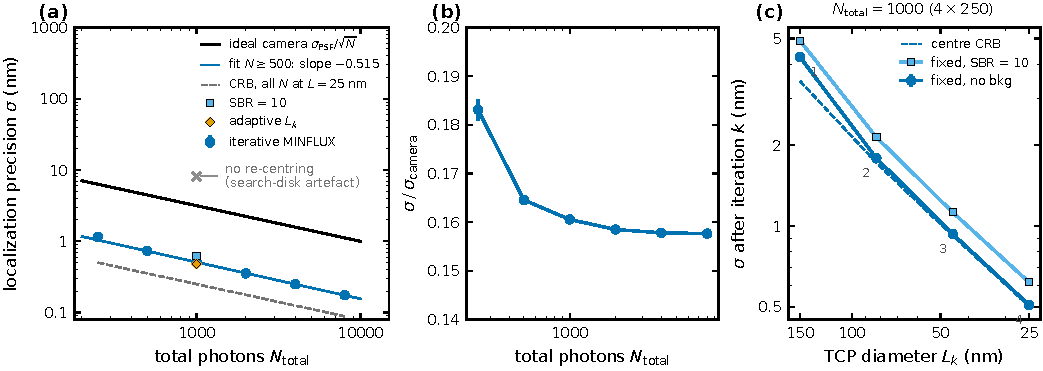
\includegraphics[width=\textwidth]{figures/fig6_iterative.pdf}
\caption{Iterative MINFLUX versus camera localization (4 iterations, $L_k=150\to25$\,nm, equal
photon split, re-centring, MLE, no background, $10^4$ repetitions). (a)~Final precision
($\sigma\pm$ bootstrap SE) versus total photon budget, with the ideal camera
$\sigma_{\mathrm{PSF}}/\sqrt N$, the fitted slope for $N_{\mathrm{tot}}\ge500$
($\pnum{iterative_slope_N_ge_500}\src{iterative_slope_N_ge_500}$), the centre CRB if all photons
were spent at $L=25$\,nm, and single points with $\sbr=10$ and with the adaptive schedule at
$N_{\mathrm{tot}}=1000$; the grey cross (no re-centring) is an artefact of the truncated search
disk. (b)~$\sigma/\sigma_{\mathrm{camera}}$ versus $N_{\mathrm{tot}}$, from
\pnum{iterative_ratio_max}\src{iterative_ratio_max} to
\pnum{iterative_ratio_min}\src{iterative_ratio_min}. (c)~$\sigma$ after each iteration versus the
pattern diameter $L_k$ for $N_{\mathrm{tot}}=1000$, without background and with $\sbr=10$,
compared with the centre CRB of each iteration.}
\label{fig:iterative}
\end{figure*}
